\scanpage{114}
\margin{\figure{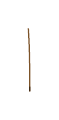
\begin{tikzpicture}
\draw[brown!65!black,line width=.45pt] (0,0) .. controls (.015,-.20) and (.02,-.55) .. (.02,-.80);
\draw[brown!35!black,line width=.45pt] (.019,-.74)--(.02,-.80);
\end{tikzpicture}}}
is moreover proper, then for \uline{every} linear subvariety $\inserted{L_t}$ of codimensio\handwritten{n} $s$, $Y_t=f_t^{-1}(L_t)$ is geometrically connected.

Combining with 2, we find, by the argument which enabled us to deduce 3 from 1 :

\margin{\handwritten{\begin{tabular}{@{}l@{}}cf.\\S\unsure{G|C}A 1 X \unsure{2.11|2,11|2,II|2.II}\end{tabular}}}
\margin{\figure{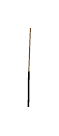
\begin{tikzpicture}\draw[brown!55!black,line width=.35pt] (.025,0)--(.005,-.55);\draw[black,line width=.55pt] (.005,-.55)--(0,-1);\end{tikzpicture}}}
\uline{Corollary} 5: \deleted{With}\inserted{\handwritten{Under}} the hypotheses of \unsure{3|4} , \inserted{with $X$ proper,} the danonical homomorphism $\handwritten{\pi}_1(Y_{\bar t})\handwritten{\rightarrow}\handwritten{\pi}_1(X)$ ($\handwritten{\simeq}\handwritten{\pi}_1(X_{\bar t})$ by the base change theorem) is surjective.

We also desire a statement analogous to 5, giving a surjectivity for $\handwritten{\pi}_1$ for a non-generic $t$, but without a properness hypothesis, and for larger quotients of $\handwritten{\pi}_1$ than those considered in (**). One can\deleted{n\unsure{t|l}} give the following result on this subject:

\margin{\figure{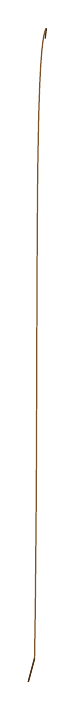
\begin{tikzpicture}
\draw[brown!65!black,line width=.45pt] (.15,0) .. controls (-.02,-.2) and (.06,-4) .. (0,-8) --(-.08,-8.3);
\draw[brown!35!black,line width=.45pt] (.15,0)--(.135,-.13);
\draw[brown!35!black,line width=.45pt] (0,-8)--(-.08,-8.3);
\end{tikzpicture}}}
\uline{Theorem} 6. Su\unsure{p|i}\unsure{p|t}ose $k$ algebraically closed, \inserted{\handwritten{and}} $X$ proper, $f:X\handwritten{\rightarrow}P^r$, \deleted{and} the linear subspace $L_t$ of $P^r$ of codimension $s$ (defined over $k$, to fix ideas) \deleted{such that we have} and finally the closed subscheme $D$ of $X$ such that we have the following; \deleted{where we have set $U=X-D$}

a) \deleted{$U_t=U\unsure{\cap}X_t$ and} $\deleted{X}\handwritten{Y}_t=f^{-1}(L_t)$ is nonempty.

b) For every $x\handwritten{\in}\deleted{X}\handwritten{Y}_t$ , $X$ is smooth at $x$, $Y_t$ is smooth at $x$\handwritten{,} of codime\unsure{m|n}tsion $s$ in $X$ at $x$, $f$ is clean at $x$.

c) For every $x\handwritten{\in}D_t=D\handwritten{\cap}Y_t$ , o\deleted{\unsure{\`{}}}r \deleted{else} else $\operatorname{codim}_x(D_t,\mathord{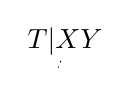
\begin{tikzpicture}[baseline=(g.base),x=1em,y=1em]\node[inner sep=0pt] (g) at (0,0) {$\deleted{\unsure{T|X}}\handwritten{Y}$};\fill[black] (-.17,-.73) ellipse (.026 and .036);\fill[brown!60!black] (-.24,-.92) circle (.03);\end{tikzpicture}}_t)\handwritten{\geqslant}2$, or else $D_{\deleted{\unsure{t}}}$ is a divisor \unsure{e|s}\unsure{n|u}r $X$ at $x$ and $\deleted{D_t}$ induces on $Y_t$ at $x$ a divisor with normal crossings.

Suppose $U=X-D$ irreducible, and consider the inclusion $U_t=U\handwritten{\cap}Y_t\handwritten{\longrightarrow}U$ . \deleted{Then $U_t$} Let $\handwritten{\pi}_1^t(U)$ be the \deleted{grou} quotient of the fundamental group of $U$ \deleted{formed of the} which classifies the coverings of $U$ which are tamely ramified at the irreducible components of codimension 1 of $D$ in $X$ which meet $Y_t$, \deleted{(\unsure{i.e.} such that $D$} and $\overset{\unsure{\scriptscriptstyle t|+}}{\handwritten{\pi}}_1^t(\unsure{U|V}_t)$ the \deleted{analogous} quotient of $\handwritten{\pi}_1(U_t)$ which classifies the coverings which are tamely ramified at the irreducible components of codimension 1 of $D_t$ . We have a homomor-
% archive sheet number: 113
